\documentclass[12pt]{article}
\usepackage[polish]{babel}
\usepackage[letterpaper,top=3cm,bottom=3cm,left=3cm,right=3cm,marginparwidth=1.75cm]{geometry}
\usepackage{amsmath}
\usepackage{amssymb}
\usepackage{graphicx}
\usepackage[colorlinks=true, allcolors=blue]{hyperref}
\usepackage{polski}
\usepackage{enumitem}
\usepackage{float}
\usepackage{tikz}
\newtheorem{lemma}{Lemat}
\newtheorem{theorem}{Twierdzenie}

\title{Indeks Chromatyczny (kolorowanie krawędzi)}
\author{Gabriel Budziński\\254609}

\begin{document}
\maketitle

\section{Opis problemu}

Jeśli $G$ jest grafem, to \textit{indeks chromatyczny} $\chi'(G)$ jest najmniejszą liczbą kolorów potrzebnych do pokolorowania jego krawędzi w taki sposób, aby sąwiadujące krawędzie (mające wspólny wierzchołek) były różnych kolorów. Od razu można zauważyć, że jeśli maksymalny stopień wierzchołka w $G$ to $\Delta$, to $\chi'(G) \geq \Delta$.

\subsection{Pozytywny przykład problemu}

Czy graf $C_4$ jest 2-kolorowalny krawędziowo?

\begin{center}
\begin{tikzpicture}
    \begin{scope}[every node/.style={circle,thick,draw}]
        \node (A) at (0,0) {};
        \node (B) at (0,3) {};
        \node (C) at (3,0) {};
        \node (D) at (3,3) {};
    \end{scope}
    
    \begin{scope}
        \path [-,red] (A) edge node {} (B);
        \path [-,green] (B) edge node {} (D);
        \path [-,green] (A) edge node {} (C);
        \path [-,red] (D) edge node {} (C);
    \end{scope}
\end{tikzpicture}
\end{center}

Graf $C_4$ jest w oczywisty sposób 2-kolorowalny krawędziowo.

\subsection{Negatywny przykład problemu}

Czy graf $C_3$ jest 2-kolorowalny krawędziowo?

\begin{center}
\begin{tikzpicture}
    \begin{scope}[every node/.style={circle,thick,draw}]
        \node (A) at (0,0) {};
        \node (B) at (1.5,2.6) {};
        \node (C) at (3,0) {};
    \end{scope}
    
    \begin{scope}
        \path [-,red] (A) edge node {} (B);
        \path [-,green] (B) edge node {} (C);
        \path [-,green] (A) edge node {} (C);
    \end{scope}
\end{tikzpicture}
\end{center}

Graf $C_4$ nie jest 2-kolorowalny krawędziowo.

\section{Historia}

Jak wiele problemów pokrewnych, kolorowanie krawędzi wywodzi się z problemu kolorowania map, przedstawionego przez Francisa Gutherie'a w 1852. Nawiązując do tego Peter Guthrie Tait pokazał jak 4-kolorowanie mapy daje 3-kolorowanie krawędzi (\textit{Tait coloring})~\cite{tait_1880}. Ponadto, proces jest odwracalny: 3-kolorowanie krawędzi daje 4-kolorowanie mapy. W 1916 roku Dénes König pokazał, że każdy graf dwudzielny o maksymalnym stopniu wierzchołka $\Delta$ może być pokolorowany za pomocą $\Delta$ kolorów~\cite{König1916}. Kolejną pracą w której ukazało się kolorowanie krawędzi napisał Claude Shannon, opisując problem oznaczania kolorami kabli przychodzących do danego punktu w sieci elektrycznej. Dowiódł on, że przewody każdej z sieci mogą być pokolorowane przy użyciu $\lfloor 3m/2 \rfloor$ kolorów, gdzie $m$ to największa liczba przewodów w jednym punkcie~\cite{Shannon1949ATO}. Znacznego zaostrzenia tego ograniczania dokonał Vadim Vizing, który w 1964 roku pokazał, że jeśli największa liczba równoległych krawędzi w multigrafie $G$ o maksymalnym stopniu $\Delta$ to $\mu$, to $\chi'(G) \leq \Delta + \mu$, co dla grafów prostych (z $\mu = 1$) oznacza, że $\chi'(G) = \Delta \lor \chi'(G) = \Delta + 1$~\cite{1571980075458819456}.

\section{NP-zupełność}

Bazując na tych odkryciach, do obliczenie $\chi(G)$ grafu prostego $G$ wytarczy `tylko' rożróżnić, czy graf jest klasy 1 ($\chi(G) = \Delta$) czy klasy 2 ($\chi(G) = \Delta + 1$). NP-zupełność tego problemu pokazał Ian Holyer~\cite{Holyer1981TheNO} w 1981 roku.

\subsection{Szkic dowodu}

Aby dowieźć NP-zupełności problemu indeksu chromatycznego, pokażemy mocniejszy wynik {-} problem stwierdzania, czy graf kubiczny (wszystkie wierzchołki o stopniu 3) ma indeks chromatyczny 3 lub 4 poprzez redukcję z 3SAT.

Weźmy zbiór klauzul $C = \{C_1, C_2, \dots, C_r\}$, zmienne $x_1, x_2, \dots, x_s$, każda z klauzul $C_i$ składa się z trzech literałów $l_{i,1},l_{i,2},l_{i,3}$, gdzie $l_{i,j}$ jest zmienną $x_k$ lub jej negacją $\bar{x_k}$.

\begin{lemma}
    Weźmy $G$ {-} graf kubiczny 3-kolorowalny, $V' \subseteq V(G)$ podzbiór wierzchołków $G$, $E' \subseteq E(G)$ zbiór krawędzi łączących $V'$ z resztą grafu. Wtedy jeśli liczba krawędzi w o kolorze $i$ w $E'$ równa się $k_i$ $(i = 1,2,3)$, to
    \[k_1 \equiv k_2 \equiv k_3(\mod2)\] 
\end{lemma}

Mając instnację $C$ problemu 3SAT pokażemy jak skonstruować graf kubiczny $G$, który jest 3-kolorowalny wtedy i tylko wtedy, gdy $C$ jest spełnialne. Zmienne będą postaci par krawędzi: para o tym samym kolorze to $T$, a o różnym $F$.

Wprowadzimy teraz komponentę inwertującą (Rys.~\ref{fig:inv_component}). Z lematu 1. możemy zobaczyć, że jeśli ta komponenta jest 3-kolorowalna, to jedna z par krawędzi $a,b$ lub $c,d$ musi mieć równe kolory, a pozostałe 3 krawędzie różne. Traktując pary $a,b$ jako wejście i $c,d$ jako wyjście, komponenta potrafi zmieniać reprezentację $T$ na $F$ i vice versa.

\begin{figure}[H]
    \centering
    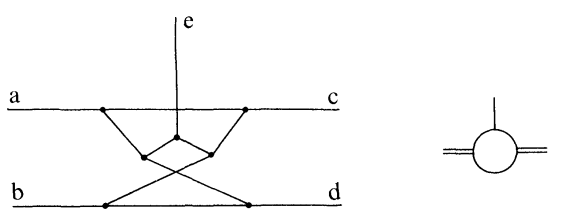
\includegraphics[scale=1]{inverting_component.PNG}
    \caption{Komponenta inwertująca}
\label{fig:inv_component}
\end{figure}

Prawdziwość każdej ze zmiennych $x_i$ będzie reprezentowana przez komponentę wartościującą (Rys.~\ref{fig:var-set_component}). Ta komponenta ma 4 pary krawędzi wyjściowych, choć w ogólności komponenta reprezentująca $x_i$ powinna mieć tyle par wyjściowych ile jest wystąpień $x_i$ i $\bar{x_i}$ w klauzulach $C$. Można pokazać, że w każdym 3-kolorowaniu komponent wartościujących wszystkie pary wyjściowe muszą przyjmować tę samą wartość.

\begin{figure}[H]
    \centering
    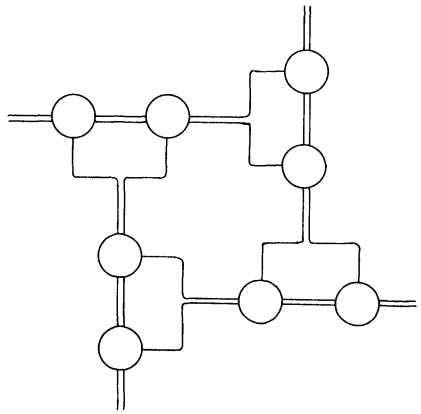
\includegraphics[scale=1]{variable-setting_component.PNG}
    \caption{Komponenta wartościująca zbudowana z 8 komponent inwertujących mająca 4 wyjścia par krawędzi. W ogólności zbudowana jest z 2n komponent inwertujących oraz ma n par wyjść}
\label{fig:var-set_component}
\end{figure}

Prawdziwość każdej z klauzul $c_j$ będzie sprawdzana przez komponętę testującą (Rys.~\ref{fig:test_component}). Ta komponenta ma 3-kolorowanie wtedy i tylko wtedy gdy nie wszystkie z par wejściowych reprezentują $F$. Pozostałe krawędzie będą omówione później.

\begin{figure}[H]
    \centering
    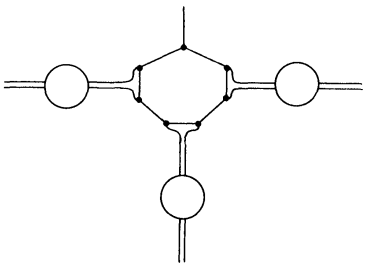
\includegraphics[scale=1]{satisfaction-testing_component.PNG}
    \caption{Komponenta testująca}
\label{fig:test_component}
\end{figure}

Mamy teraz narzędzia do dowodzenia następującego tweirdzenia.

\begin{theorem}
    Wyznaczenie czy indeks chromatyczny grafu kubicznego to 3 lub 4 jest problemem NP-zupełnym.
\end{theorem}

Pokażmy wielomianową redukcję z problemu 3SAT. Weźmy instancję 3SAT $C$ i skonstruujmy z niej graf $G$ w następujący sposób.

Dla każdej zmiennej $x_i$ zbudujmy komponentę wartościującą $X_i$ z jedną parą krawędzi wyjściowych dla każdego wystąpienia $x_i$ lub $\bar{x_i}$ w klauzulach $C$. Zbudujmy także komponętę testującą $C_j$ dla każdej z klauzul $c_j$. Załóżmy, że literał $l_{j,k}$ z klauzuli $c_j$ to zmienna $x_i$. W takim wypadku połączmy $k$-tą parę wejściową $C_j$ z odpowiednim wyjściem $X_i$. W przypadku kiedy $l_{j,k}$ to $\bar{x_i}$ wstawmy komponentę inwertującą pomiędzy $k$-tą parą wejściową $C_j$ a odpowiednią parą w $X_i$. Graf wynikowy $H$ ma pewne niepołączone krawędzie. Graf kubiczny $G$ jest zbudowany z dwóch kopii $H$ łącząc pozostałe krawędzie w pary.

Graf $G$ ma 3-kolorowanie krawędziowe wtedy i tylko wtedy, gdy $C$ jest spełnialne. Ponadto, graf $G$ jest konstruowany z $C$ w czasie wielomianowym, co dowodzi tezie.

\section{Warianty problemu}

\subsection{Grafy planarne}

Dla grafów planarnych o $\Delta(G) \geq 8$ Vizinig~\cite{1571980075458819456} pokazał
\[\chi'(G) = \Delta(G)\]
Później~\cite{SANDERS2001201} pokazano wynik silniejszy: Dla grafów planarnych o $\Delta(G) \geq 7$
\[\chi'(G) = \Delta(G)\]

\subsection{Grafy dwudzielne}

Dla grafów dwudzielnych pokazano~\cite{König1916}
\[\chi'(G) = \Delta(G)\]

\subsection{Kolorowanie acykliczne}

Acyklicznie $k$-kolorowanie krawędziowe grafu $G$ to takie $k$-kolorwanie krawędziowe, w którym krawędzie każdego z cykli mają conajmniej 3 kolory (nie ma cyckli bichromatycznych). Najmniejsze takie kolorowanie grafu $G$ oznaczamy $\chi_a'(G)$.

\subsection{Kolorowanie gwiazdowe}

\begin{itemize}
    \item Niedozwolone są cykle bichromatyczne o długości 4
    \item Najmniejsze $k$, dla którego istnieje $k$-kolorowanie gwiazdowe grafu $G$ oznaczamy $\chi_{st}'(G)$
    \item Nazwa pochodzi od wersji wierzchołkowej tego problemu.
\end{itemize}

\section{Aproksymacje}

Jako, że dla grafów prostych $\chi'(G) = \Delta(G) \lor \chi'(G) = \Delta(G) + 1$~(\cite{1571980075458819456}) to w wielomianowym czasie możemy znaleźć $\Delta(G)$, a następnie zachowawczo odpowiedzieć $\chi'(G) = \Delta(G) + 1$. Dla tego algorytmu $A$ mamy $|c_A(x) - c_{OPT}(x)| \leq 1$, a w grafie $G$, gdzie $|E(G)| \geq 1$ (nie ma sensu rozważać kolorowania krawędziowego w grafie bez krawędzi) wspołczynnik aproksymacji tego algorytmu wynosi $\frac{1}{2}$.

Aproksymacje rozważa się dla multigrafów, w których jak wspomnieliśmy Shannon~\cite{Shannon1949ATO} oraz Vizing~\cite{1571980075458819456} pokazali odpowienio $\chi'(G) \leq \lfloor \frac{3}{2}\Delta(G) \rfloor$ oraz $\chi'(G) \leq \Delta(G) + \mu$, gdzie $\mu$ to największa liczba równoległych krawędzi w $G$. Z tego dostajemy górne ograniczenia na indeks chromatyczny. Ten problem rozpatrzony jest w tej~\cite{10.1007/11427186_53} pracy.

\bibliography{bibliography}
\bibliographystyle{ieeetr}

\end{document}